% Масштабирование вычислений на суперкомпьютере.
\subsection{Масштабирование вычислений на поверхностной не- структурированной расчетной сетке}

\subsubsection{Организация межпроцессных обменов}

\begin{figure}[ht]
\centering
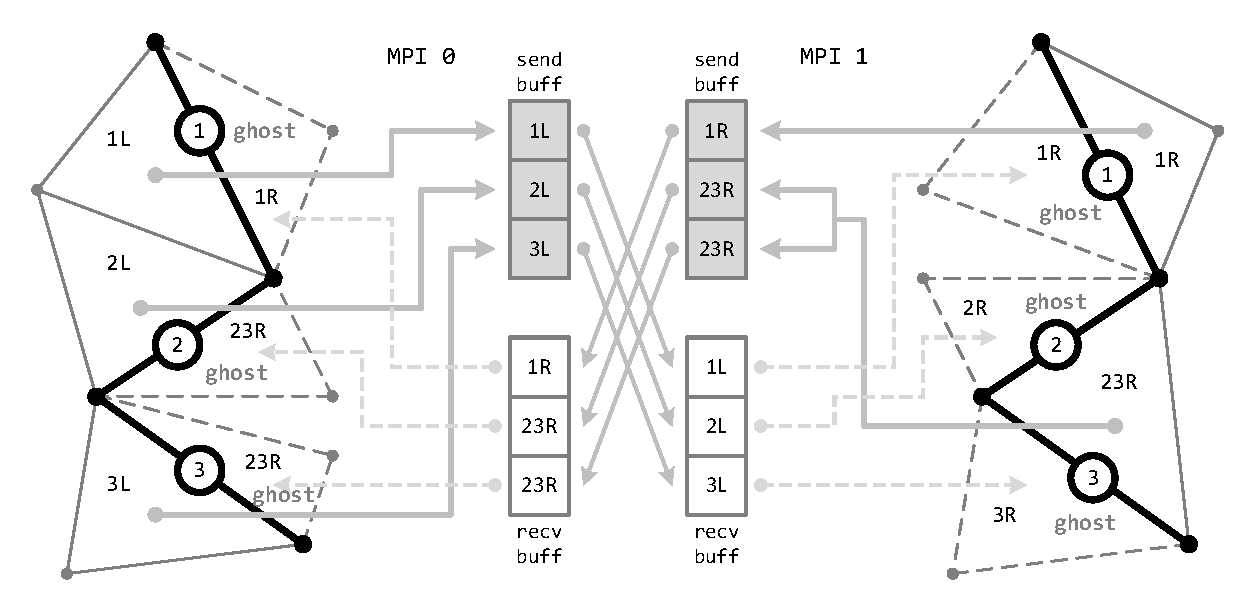
\includegraphics[width=1.0\textwidth]{pics/text_2_scaling/mpi.pdf}
\captionstyle{center}\caption{Схема выполнения MPI-обменов через границу двух доменов.}\label{fig:text_2_scaling_mpi}
\end{figure}

При проведении расчетов на декомпозированной сетке на каждой итерации счета необходимо выполнять обмен данными на каждой границе между доменами.
В нашем случае при выполнении декомпозиции расчетной сетки граница между двумя доменами представлена произвольным набором междоменных ребер.
При этом граница может быть разрывной, она и вовсе может состоять из отдельных ребер, поэтому последовательность междоменных ребер при описании границы не имеет значения.

На рис.~\ref{fig:text_2_scaling_mpi} представлена схема организации межпроцессных обменов.
На этой иллюстрации два домена (будем условно их называть левым и правым), обрабатывающиеся в MPI-процессах с номерами 0 и 1, разделены границей, состоящей из трех ребер.
При этом в левом домене присутствует три ячейки, которые примыкают к рассматриваемой границе, в правом домене таких ячеек только две (так как ячейка 23R примыкает сразу к двум ребрам границы).
Для организации межпроцессных обменов в каждом домене для каждого ребра рассматриваемой границы создаются фиктивные ячейки, которые участвуют при расчете потоков через ребра границы.
При этом пересчет физических величин в фиктивных ячейках выполнять не требуется, все данные для фиктивных ячеек получаются с помощью MPI-обменов из настоящих ячеек соседнего домена.

Для пересылки данных из настоящих граничных ячеек домена в фиктивные ячейки соседнего домена в каждом из двух соседних доменов организуются буферы отправки и приема данных.
Последовательность обмена данными выглядит следующим образом (схема показана на рис.~\ref{fig:text_2_scaling_mpi}).
Сначала данные из настоящих граничных ячеек записываются в соответствующие буферы отправки данных (send buff), далее для всех границ расчетной сетки выполняются асинхронные команды \texttt{MPI\_Irecv} приема сообщений в буферах получения данных (recv buff).
После чего также одновременно для всех границ расчетной сетки выполняются команды асинхронной отправки данных \texttt{MPI\_Isend} из буферов отправки.
Далее выполняется ожидание завершения всех асинхронных обменов данными с помощью функции \texttt{MPI\_Waitall}.
Последним шагом, завершающим обмен данными между соседними доменами, является перенос полученных физических значений из буферов получения данных (recv buff) в соответствующие фиктивные ячейки.

Можно отметить, что при использовании фиктивных ячеек возможно некоторое дублирование данных.
Например, на представленной схеме ячейке 23R из правого домена соответствуют сразу две фиктивные ячейки в левом домене.
Эти ячейки содержат одинаковые данные.
Данное дублирование информации является приемлемым, так как данные фиктивных ячеек используются только на чтение для выполнения вычисления потоков через границу доменов, поэтому в данном случае выполнять какую-либо синхронизацию одинаковых фиктивных ячеек не нужно.

\subsubsection{Эффективность масштабирования вычислений на суперкомпьютере}

Для замеров показателей масштабируемости вычислений на неструктурированной поверхностной расчетной сетке была использована тестовая поверхность обтекаемого трехмерного тела, содержащая порядка $2 \cdot 10^5$ узлов и $4 \cdot 10^5$ ячеек.
В ячейках выполнялись расчеты, связанные с моделирование течения жидкой пленки, решением уравнений теплового баланса на поверхности, а также перестроение и сглаживание поверхности.
Для декомпозиции поверхностной сетки использовался простой иерархических алгоритм деления доменов пополам, описанный в разделе \ref{sec:text_2_decompsurf_hierarchical}, в котором в качестве признаков ячеек брались три координаты центра.
При этом в результате критерием выбора конкретной координаты для деления домена являлась минимизация длины границы между двумя доменами (такой подход позволяет выполнять деление домена по наиболее протяженному направлению).

\begin{table}[!h]
\centering
\setcaptionmargin{0mm}
\onelinecaptionsfalse
\captionstyle{flushleft}
\caption{Конфигурации узлов суперкомпьютера МВС-10П, на которых производились замеры масштабирования вычислений.}
\bigskip
\begin{tabular}{|c|c|c|c|c|}
\hline
\makecell{Семейство \\
процессоров \\
Intel} & \makecell{Количество\\процессоров\\/ ядер\\/ потоков} & \makecell{Частота\\процессора} & \makecell{Объем\\оперативной\\памяти} & \makecell{AVX-512} \\
\hline\hline
Broadwell & 2 / 32 / 64 & 2,6 ГГц & 128 ГБ & нет \\
\hline
Phi KNL & 1 / 72 / 288 & 1,5 ГГц & 96 ГБ & да \\
\hline
Skylake & 2 / 36 / 72 & 3,0 ГГц & 192 ГБ & да \\
\hline
Cascade Lake & 2 / 48 / 96 & 3,0 ГГц & 192 ГБ & да \\
\hline
\end{tabular}
\label{tbl:text_2_scaling_supercomputers}
\end{table}   

Для измерения показателей масштабируемости вычислений использовались гомогенные сегменты вычислительной системы МВС-10П.
Всего расчеты проводились на четырех вычислительных сегментах, характеристики узлов которых приведены в таблице~\ref{tbl:text_2_scaling_supercomputers}.
В этой таблице можно отметить, что все микропроцессоры кроме Intel Xeon Broadwell поддерживают набор инструкций AVX-512, позволяющий использовать специальные 512-битные векторные регистры для эффективной векторизации кода.
Также следует выделить вычислительные узлы на базе микропроцессора Intel Xeon Phi KNL.
Эти микропроцессоры отличаются огромным количеством вычислительных ядер, каждое из которых способно выполнять до 4 потоков, что позволяет эффективно распараллеливать расчетные приложения вплоть до 288 потоков на одном микропроцессоре.

\begin{figure}[ht]
\centering
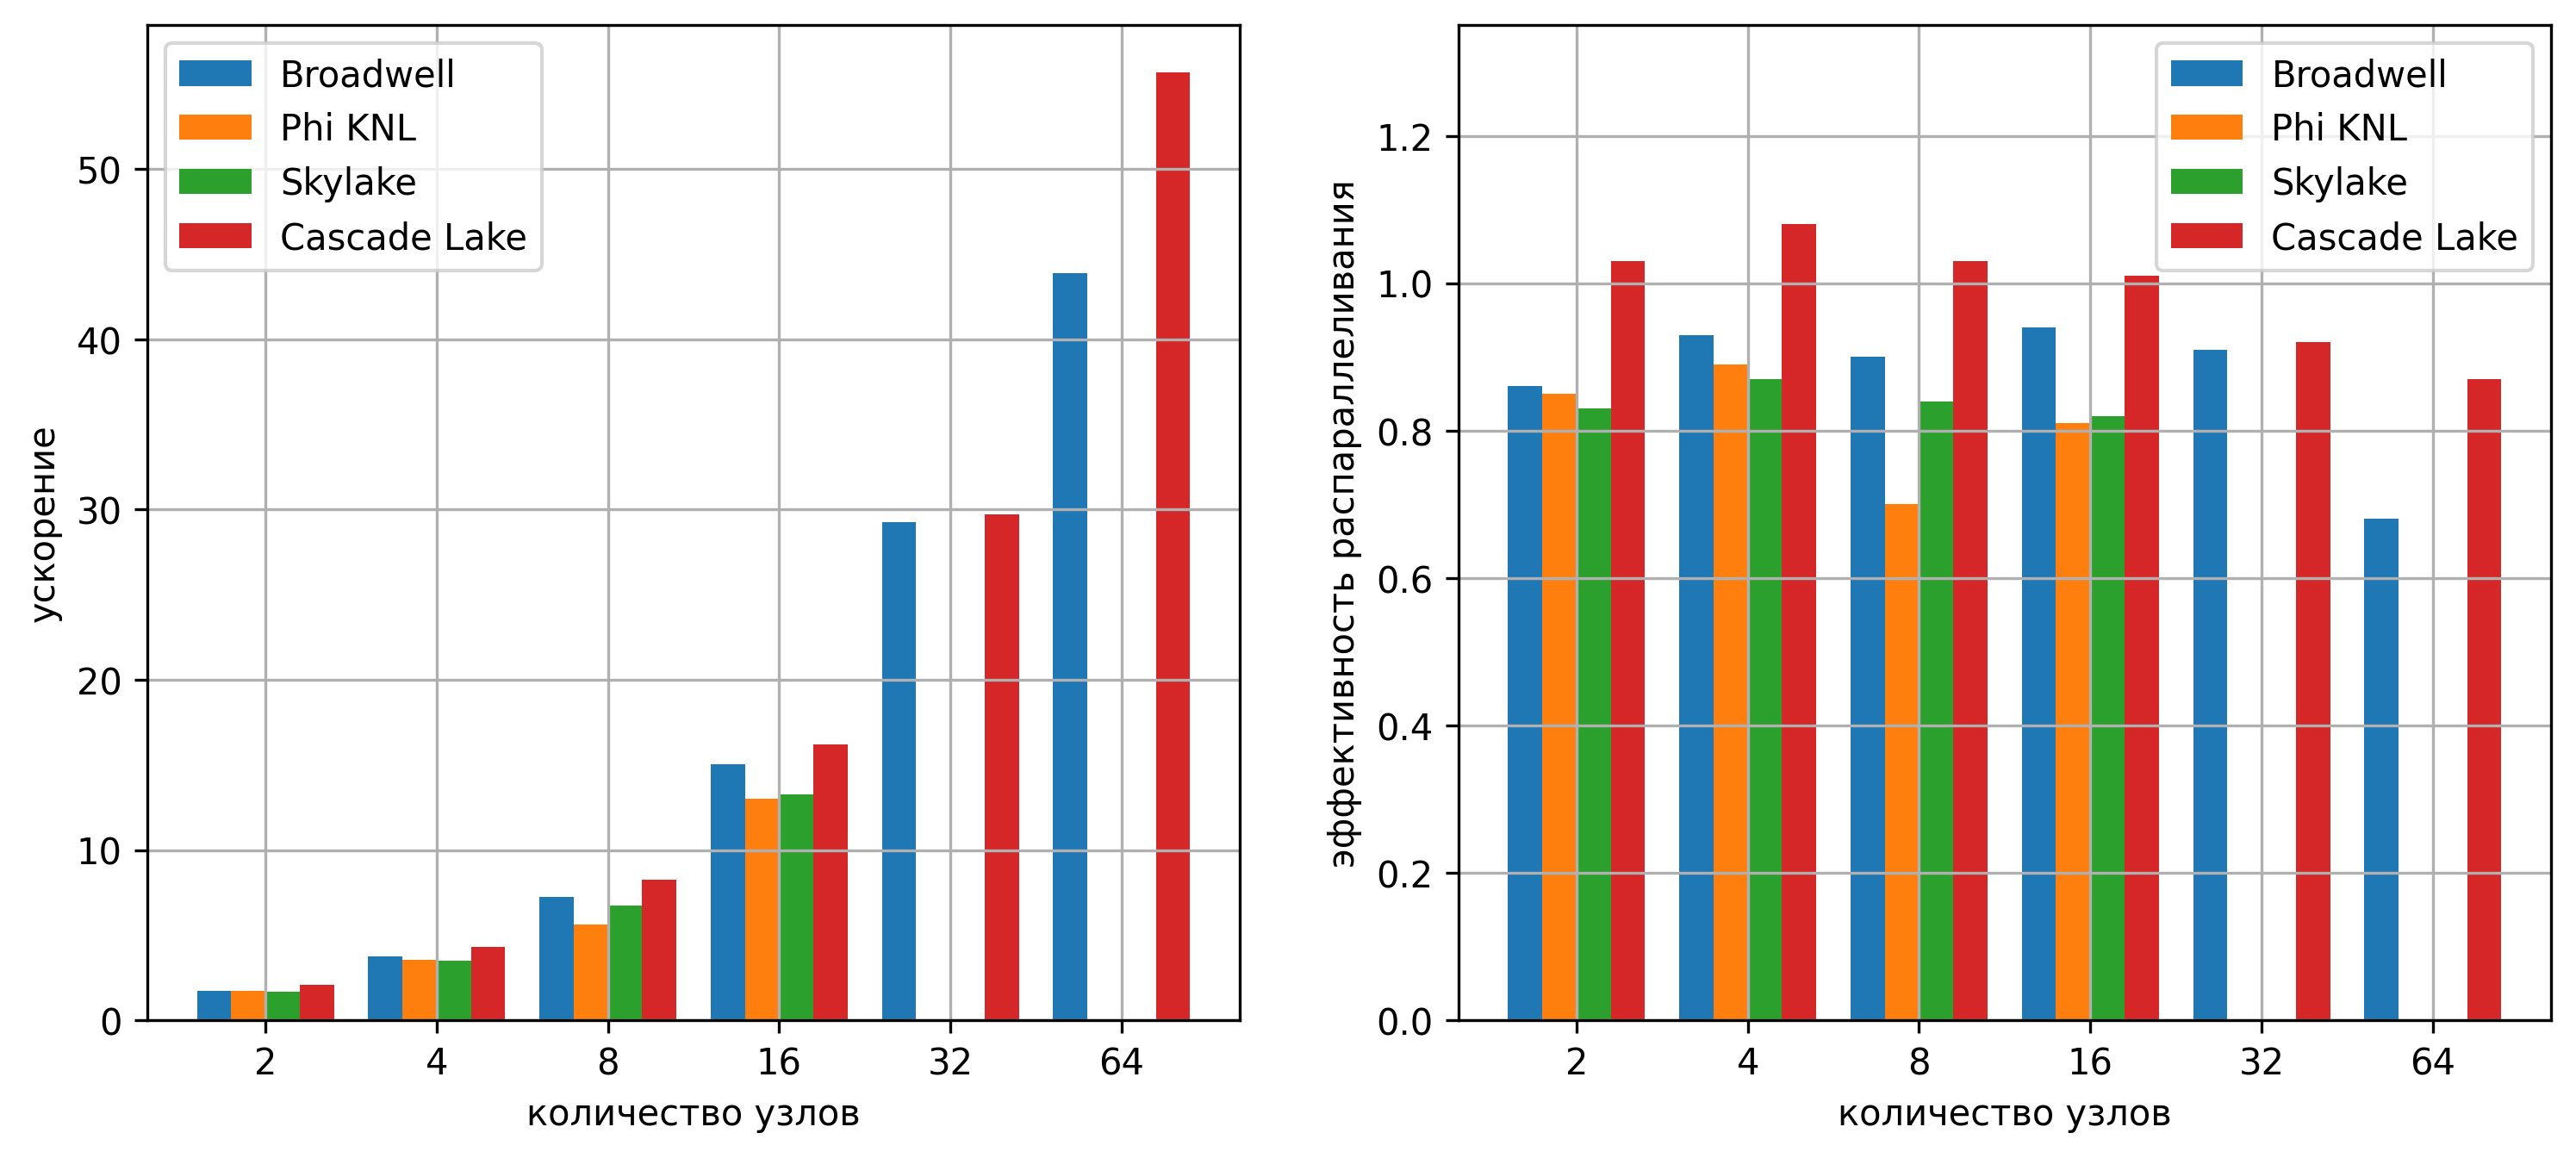
\includegraphics[width=1.0\textwidth]{pics/text_2_scaling/2in1.png}
\captionstyle{center}\caption{Ускорение (слева) и эффективность распараллеливания (справа) вычислений на сегментах суперкомпьютера МВС-10П при увеличении количества узлов.}
\label{fig:text_2_scaling_speedup_eff}
\end{figure}

Основной целью выполняемых запусков было проведение замеров показателей сильной масштабируемости вычислений при полном распараллеливании внутри вычислительных узлов с использованием OpenMP.
То есть для всех запусков использовалась одна и та же поверхность (которая дробилась на нужное количество вычислительных узлов), а также в расчетах были задействованы все потоки, доступные внутри вычислительных узлов.

При проведении расчетов замеры выполнялись независимо для каждой вычислительной системы в отдельности.
На рис.~\ref{fig:text_2_scaling_speedup_eff} приведены диаграммы ускорения вычислений $s_{msg}$ и эффективности распараллеливания $e_{msg}$ при увеличении количества вычислительных узлов для разных вычислительных систем.
Можно видеть, что для всех вычислительных систем эффективность масштабирования варьируется в районе значений 0,8-0,9, хотя на некоторых конфигурациях запуска наблюдаются провалы даже в район 0,7.
Запуски с низким значением эффективности распараллеливания как правило связаны с разбросом времени обработки MPI процессами своих доменов.
Заметим, что для сегмента Cascade Lake при количестве узлов 2, 4, 8 и 16 наблюдается проявление сверхлинейной масштабируемости (когда значение $e_{msg}$ поднимается выше единицы), однако это скорее исключение, чем ожидаемый эффект.

Несмотря на то, что использованный в запусках алгоритм декомпозиции расчетной сетки обеспечивал равномерное распределение ячеек по доменам, само время обработки ячейки сильно зависит от ее физических свойств и может отличаться в разы.
По этой причине сбалансировать вычислительную нагрузку на разные вычислительные узлы возможно только в динамическом режиме, что не делалось в рамках данного исследования.
Также отметим высокие показатели эффективности масштабирования вычислений для вычислительных узлов на базе микропроцессоров Xeon Cascade Lake.
